%%% Part dient dazu, zb. die Arbeit nochmal zu Gliedern (Einleitung, Theorieteil, ...)
\part{Part}

% neues Kapitel
\chapter{Chapter}

Always make a short intro to chapters or sections.

%neue Section
\section{Section}
\label{erstesLabel}

some intro words \dots

% NICHT TIEFER ALS SUBSECTION!!!
\subsection{SubSection}
\label{zweitesLabel}

First label was set in section \ref{erstesLabel} - the second in section \ref{zweitesLabel}.

Remember: Always reference any figures or tables within the prose text!

A reference will be done like this: \cite{keyToBibEntry}

Do not cite things like Wikipedia, Slides, etc (only Books and scientific papers allowed - or W3C Recommendations \cite{w3c_example} and articles on trusted sites marked with a date and an corresponding author)

Please code URLs like this: \url{http://www.google.de}

If you name projects like A.I.R\footnote{\url{https://www.dimis.fim.uni-passau.de/iris/index.php?view=air} -- last checked: \today} or Eclipse\footnote{\url{http://www.eclipse.org/} -- last checked: \today} or whatever, use footnotes to cite the URL.

%Example Figure
\begin{figure}[H]
	\begin{center}
		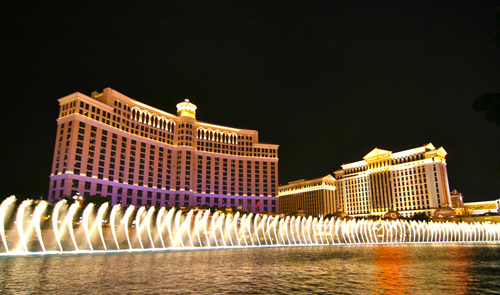
\includegraphics[width=0.75\textwidth]{holiday.png}
	\end{center}
	\caption{After the thesis it's time for holiday}
	\label{labelToRef}
\end{figure}

%Example Itemize
\begin{itemize}
	\item item 1
	\item item 2
	\item lala
\end{itemize}

%Example Description
\begin{description}
	\item[item 1] is needed in order to blabla
	\item[item 2] defines blabla
	\item[lala] lala
\end{description}

% Example Definition
\begin{Def}[Title]
\label{key}
Description \dots
\end{Def}

% Example Table
\begin{table}[H]
\begin{center}
\caption{Caption of the table}
\label{lalala}
\begin{tabular}{| l | l |}
\hline
first column & second column \\
\hline
\hline
\dots & \dots \\
\hline
\dots & \dots \\
\hline
\end{tabular}
\end{center}
\end{table}

\begin{procedure}[ht]        
\caption{Greedy Heuristic()} 
\label{greedy}        
\KwData{request profile $Q$, backends $B$} 
\KwResult{allocation schema}

sort(request profile $Q$) according cost function $c_S$ descending \; 

\ForEach{$C \in Q$}{

   \ForEach{$b \in B$}{
      \eIf{$b.free\_capacity > 0$} {
      $UNION \leftarrow b.relations \cup C.relations$\;
      $INTERSECT \leftarrow b.relations \cap C.relations$\;
      ${diff}[C,b] \leftarrow c_S(INTERSECT) - c_S(UNION)$\;
      }
      {$diff[C,b] \leftarrow -\infty$;}
   }
   
   \While{$C.rest\_workload > 0$}{
      
      $b \leftarrow b \in B \mbox{ where } diff[C,b]  \mbox{ maximal}$\;
      
      $workload\_for\_b \leftarrow \min({b.free\_capacity, C.rest\_workload})$\;
      
      $b.add(C , workload\_for\_b)$\;
      
      $C.rest\_workload \leftarrow C.rest\_workload - workload\_for\_b$\;
      
      
      ${diff}[C,b] \leftarrow -\infty$;
      
   }
}
\end{procedure}
